

\section{历史}

\begin{figure}[H]
	\centering
	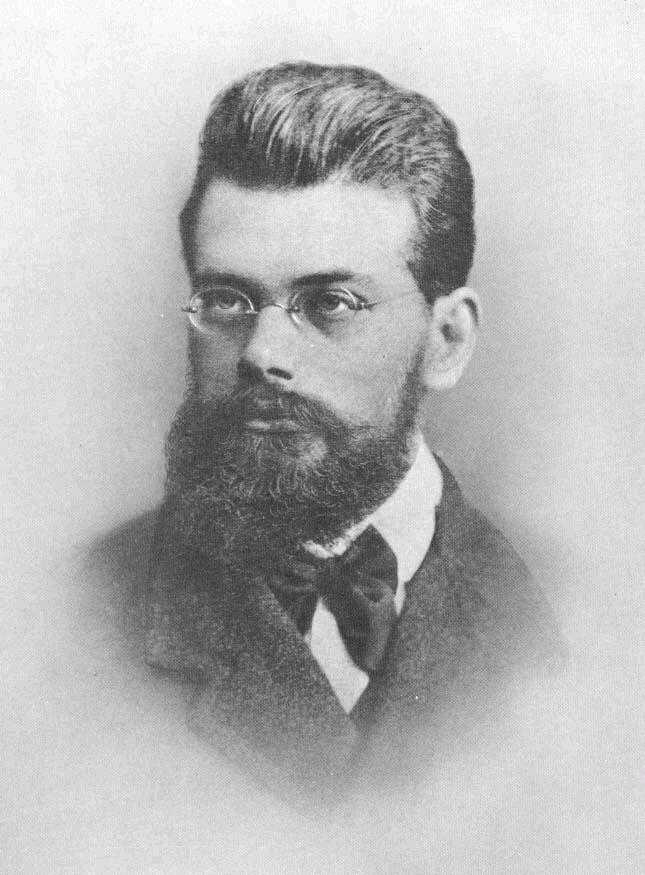
\includegraphics[width=\linewidth/2]{pic/bolzman.jpg}
	\caption{玻尔兹曼}
	\label{fig:results}
\end{figure}


1872年,Ludwig Boltzmann在维也纳科学院的会议报告上发表了著名的《Weitere Studien über das Wärmegleichgewicht unter Gasmolekülen》(Further Studies on the Thermal Equilibrium of Gas Molecules)其中他引入了量

\begin{equation}
  H(t)=\int_0^\infty f(E,t)[\ln \frac{f(E,t)}{\sqrt{E}}-1]   dE
\end{equation}

并证明了  必定随时间单调递减,且在  为Boltzmann分布时达到极小值。这个证明相当困难,Boltzmann只完成了在离散状态下的求解。至此一生饱受攻击,终于1906年在意大利Duino海滩自杀。而主要攻击他的论点分为Loschmidt悖论与Zermolo悖论。


\section{Loschmidt悖论}
Boltzmann最初的研究对象是气体分子,而气体分子遵循的经典动力学理论是时间反演对称的,这显然与H定理里蕴含的时间方向的不对称是矛盾的。

这个观点首先由William Thomson在1874年提出\cite{1}

很有意思的是,Willams Thomson是提出热寂说的人,而这个悖论里的人Josef Loschmidt恰是反对热寂说的

\begin{quote}
	He sought to destroy the terrifying nimbus of the second law, which has made it appear as a principle of destruction for all living creatures in the universe; and at the same time, to open up the comforting prospect that the human race does not depend upon coal or the sun to transform heat into work, but may have an inexhaustible supply of transformable heat.
\end{quote}

而且Loschmidt首次提到时间反演对称正是在1876年他在论文《Über den Zustand des Warmegleichgewichtes eines Systems von Körpern mit Rucksicht auf die Schwerkraft》(The State of Thermal Equilibrium of a System of Bodies with Regard to Gravity.)中提到的。Boltzmann要被对第二定律持不同态度的学者同时攻击,这也的确挺惨的。

但事实上他和Loschimidt是很好的朋友,所以Boltzmann紧接着在1877年发表《Uber die Beziehung eines allgemeine mechanischen Satzes zum zweiten Hauptsatze der Warmetheorie》(On the Relation of a General Mechanical Theorem to the Second Law of Thermodynamics  )怼了回去,他的核心观点是,以均匀分布为平衡态为例,并不是所有的初始状态都能演化到均匀分布,我们也永远没法证明这一点;但能演化为均匀分布的初始状态数量远大于演化到非均匀的。很明显在这里Boltzmann已经有了系综和对第二定律的概率性理解。

\section{Zermelo悖论}
其实这个思想是出自于法国人Henri Poincaré,他1893年的论文《Le mécanisme et l'expérience》(Mechanism and Experience)提到了这个点(届时距离他提出Poincaré猜想还有11年)。

\begin{quote}
	The world does not remain that way forever, if the theorem cited above is not violated; it merely stays there for an enormously long time, a time which is longer the more numerous are the molecules.
\end{quote}

然而他所用的著名的Poincaré reccurence定理是他首次在1890年讨论三体问题的动力学方程时证明的\cite{2}

更加普适的表达要到1902年Lebesgue引入测度论作为合适的数学语言,在1919年才被Constantin Carathéodory严格证明。

我们先看看Poincaré reccurence theorem的内容

Let $T:(X,B,m) \rightarrow (X,B,m)$ be a measure-preserving transformation, then for all $B \subset B$ such that $m(B)>0$,there exists  $F \subset B$ such that  $m(F)=m(B)$ and for all $x \in F$, there exists  $0<n_1<n_2<\cdots$ satisfying $T^{n_i }(x) \in F, \forall i \in \mathbbm{N}$ .


即任意的集合 ,其中在保测变换的迭代下无法做到无限次回到  的集合是零测的。通俗的讲,几乎所有的状态点在保测变换的迭代下会无限次返回初始状态点附近。这是保测映射内蕴的性质,而Liouville定理(Liouville方程在1838年就得到了)告诉我们在相空间上哈密顿流是保体积不变的,那么经典动力系统必然是满足Poincaré回复定理的。

1896年,德国人Ernst Zermelo还在柏林跟Max Planck学物理,距离他发表最为人熟知的Zermelo定理(二人完全信息博弈必存在不败解)还有27年。他把Poincaré的三体问题推广到了多体,得到了类似的结果,于是对Maxwell、Boltzmann和同样支持H定理的Lorentz都批判了一番。他的观点是:在不指定初始条件的情况下,我们是不可能证明系统按照第二定律预测的方向演化的。其实我们可以看到此处Zermelo还是在考虑一个绝对确定体系的问题,事实上如果有系综的概念以及对第二定律的概率性的理解的话,他这个观点就非常naive了。所以Boltzmann自然不留情面,1896同年就给了一个非常尖锐的回复:你讲的Poincaré定理显然是对的,但你不会用,你根本就误解了我讲的H定理!

\begin{quote}
	The Poincare theorem is of course inapplicable to a terrestrial body which we can observe, since such body is not completely isolated; likewise, it is inapplicable to the completely isolated gas treated by the kinetic theory, if one first lets the number of molecules become infinite, and then the quotient of the time between successive collisions and the time of observation becomes zero.
\end{quote}

Boltzmann的嘲讽:

\begin{quote}
	He is just like a dice player who has calculated that the probability of a sequence of 1000 one's is not zero, and then concludes that his dice must be loaded since he has not yet observed such a sequence!
\end{quote}

至此其实我们已经很好理解了,Boltzmann的核心观点就一个——你们讲时间反演对称是没错,Poincaré重现也没错,但这些情况都是少数,相比之下满足我的H定理的初始状态是一个overwhelming的大数!

\section{解决悖论}

1906年,Boltzmann在意大利Duino海滩和妻女度假的时候自缢身亡。两年之后,原子被证明真实存在(Ernest Rutherford),物理学家们最终承认了Boltzmann的观点。但在数学上大部分人并不接受,按照Boltzmann的原始说法,可以说H定理只是依概率成立的。这实际上是因为Boltzmann没有合适的数学语言去表达。到50年代大家才开始试着做H定理的严格化。1949年Harold Grad在Communications on pure and applied mathematics发表的文章里提到了\cite{3}

\begin{quote}
	First, from equilibrium considerations we must let the number density of molecules,$N$,increase without bound. At the same time we would like the macroscopic properties of the gas to be unchanged. To do this we allow in to approach zero in such a way that $mN=\rho$is fixed.
\end{quote}

这其实是热力学极限最早的体现形式之一,在当时称作Boltzmann-Grad极限。杨振宁李振道著名的考虑热力学极限下的相变严格解的工作也是在1952年了。而我们回顾Boltzmann的解释,他将其归因于在宏观极小的体积内,也必定有几乎无限多的分子,在这样的情况下,H定理是成立的;在当时大部分人不理解Boltzmann为什么可以在持有这种观点的同时承认无论基本粒子有多小,总归是有限多的。其实这并不矛盾,因为他知道在非热力学极限的情况下肯定是存在涨落的。事实上这就是同一个意思,可惜Boltzmann的数学素养没有好到表述得令人信服,以至于一生里花掉大量的时间去为与人争斗。到60年代,用计算机做MD模拟流行起来,也很好地证实了H定理。再到70年代有了形式化的表达:

If $f(p_1,q_1;\cdots,p_N,q_N)=\prod_{i=1}^N f(p_i,q_i)$,then $f$ will be a solution of Boltzmann equation asymptotically with  $N \rightarrow \infty$ and $\rho$ remains finite. In particular,$H$ will be a monotonically decreasing function of time in the same limit.

但要给出严格的分析的证明其实是非常非常困难。
然而1975年Oscar Lanford给出了一个弱化的证明\cite{4}

在极小的时间区间内(约1/5平均碰撞时间量级)考虑H定理是严格成立的。
至此H定理介绍告一段落,关于Boltzmann方程和非平衡态的细节以后慢慢补。

\section{关于量子力学}
事实上Gibbs对H定理的理解也很独到,由Liouville定理我们知道哈密顿流在相空间中的演化是保体积的,但Gibbs从量子力学的角度出发来考虑,他认为在相流的演化过程中会出现dendritic形状,其中树突之间的距离足够近以至于到了$h$的尺度之后就无法从宏观上做出区分了,宏观上来看,相流的密度减少而体积增大了,这是对H定理另一种层面的理解。

\section{注记}
H定理和Boltzmann方程与非平衡态统计物理有非常密切的联系,事实上至今还是比较Open的问题,2017在arXiv的这篇论文即是探讨Boltzmann熵,Gibbs的粗粒化熵细粒化熵的关系,作者声称给出了非平衡哈密顿系统的统计力学熵的定义。\cite{5}

关于H定理更详细的历史和发展,Stephen Brush的书有很丰富的内容\cite{6}。

意大利数学家Carlo Cercignani的书非常不错,他同时也对多原子体系H定理的证明做了极大贡献\cite{7}。
